
\section{OPIL Data Model}\label{sec:model}

The section describes the OPIL data model in detail.  
OPIL classes are in general organized in pairs, one for specifying the interface to a protocol, the other for making requests to execute protocol via that interface.
As such, this section is also organized in pairs, first each interface class, then the complementary request class.

\todo[inline]{remove Media and Strain classes}


\subsection{ProtocolInterface}
\label{sec:ProtocolInterface}

\begin{figure}[ht]
\begin{center}
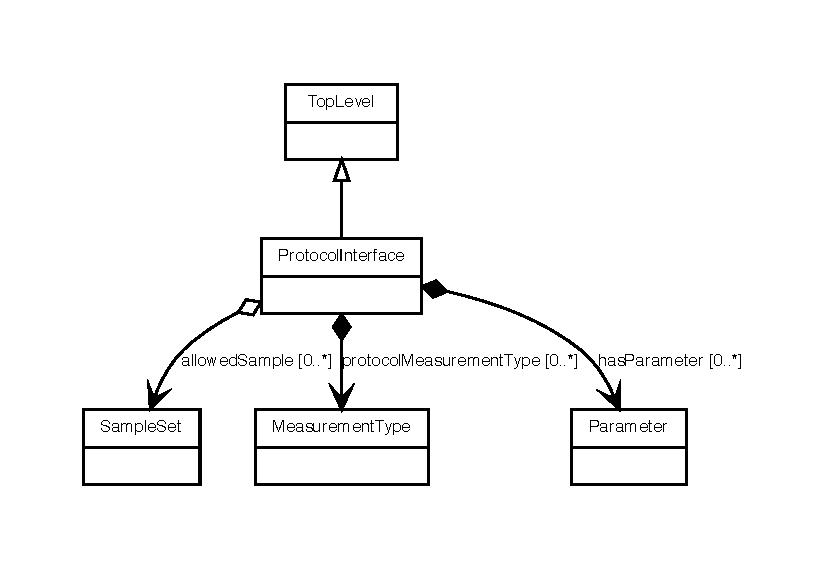
\includegraphics[scale=0.6]{figures/ProtocolInterface}
\caption[]{Diagram of the \opil{ProtocolInterface} class and its associated properties}
\label{uml:ProtocolInterface}
\end{center}
\end{figure}


\subsection{ExperimentalRequest}
\label{sec:ExperimentalRequest}

\begin{figure}[ht]
\begin{center}
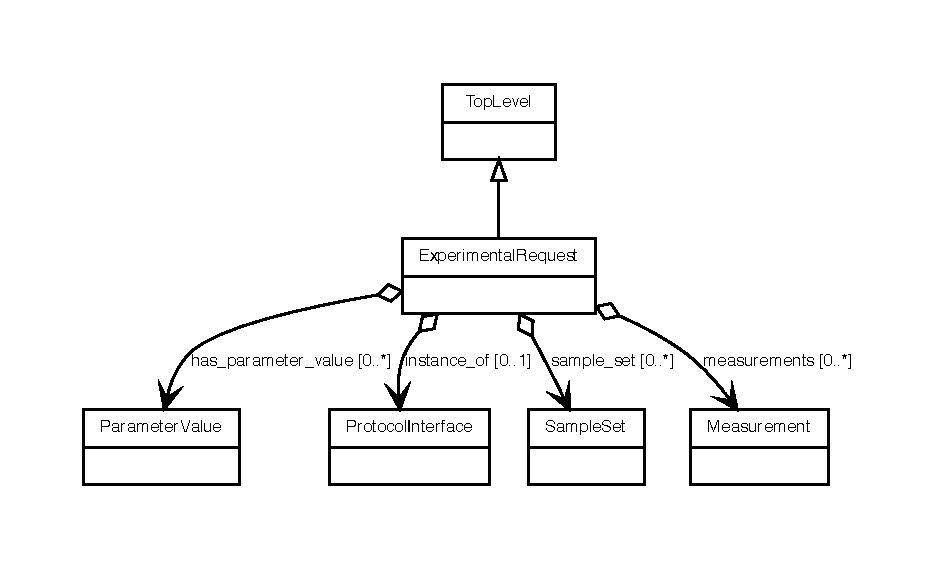
\includegraphics[scale=0.6]{figures/ExperimentalRequest}
\caption[]{Diagram of the \opil{ExperimentalRequest} class and its associated properties}
\label{uml:ExperimentRequest}
\end{center}
\end{figure}


\subsection{SampleSet}
\label{sec:SampleSet}

\begin{figure}[ht]
\begin{center}
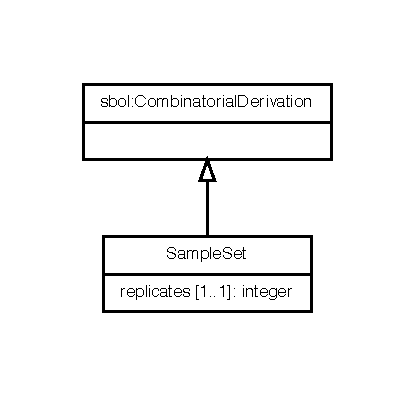
\includegraphics[scale=0.6]{figures/SampleSet}
\caption[]{Diagram of the \opil{SampleSet} class and its associated properties}
\label{uml:SampleSet}
\end{center}
\end{figure}


\subsection{Parameter}
\label{sec:Parameter}

\begin{figure}[ht]
\begin{center}
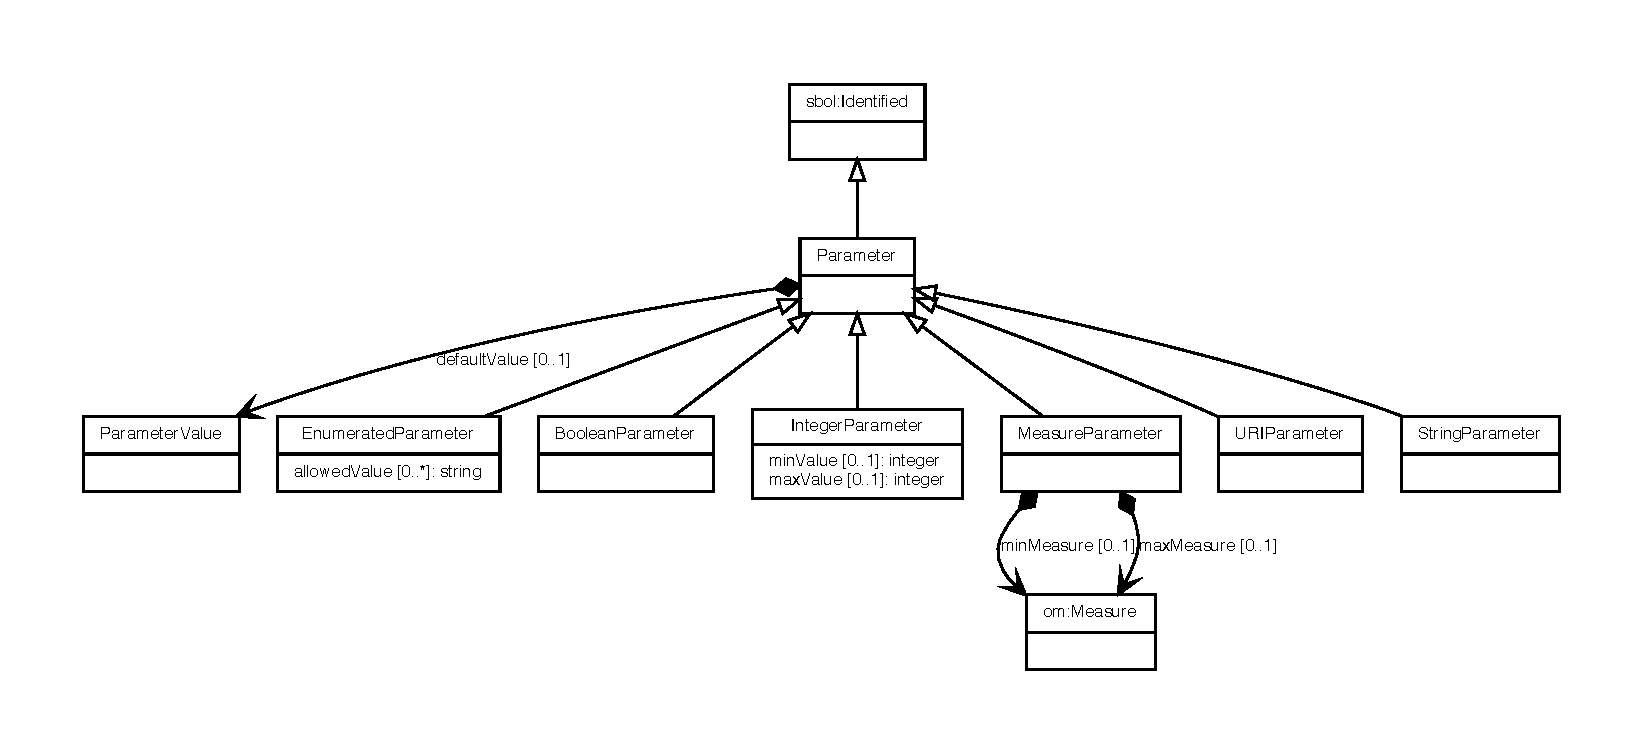
\includegraphics[scale=0.6]{figures/Parameter_definition_and_abstraction}
\caption[]{Diagram of the \opil{Parameter} abstract class and its associated properties and subclasses}
\label{uml:Parameter}
\end{center}
\end{figure}

\subsubsection{BooleanParameter}
\label{sec:BooleanParameter}

\subsubsection{EnumeratedParameter}
\label{sec:EnumeratedParameter}

\subsubsection{IntegerParameter}
\label{sec:IntegerParameter}

\subsubsection{MeasureParameter}
\label{sec:MeasureParameter}

\subsubsection{StringParameter}
\label{sec:StringParameter}

\subsubsection{URIParameter}
\label{sec:URIParameter}


\subsection{ParameterValue}
\label{sec:ParameterValue}

\begin{figure}[ht]
\begin{center}
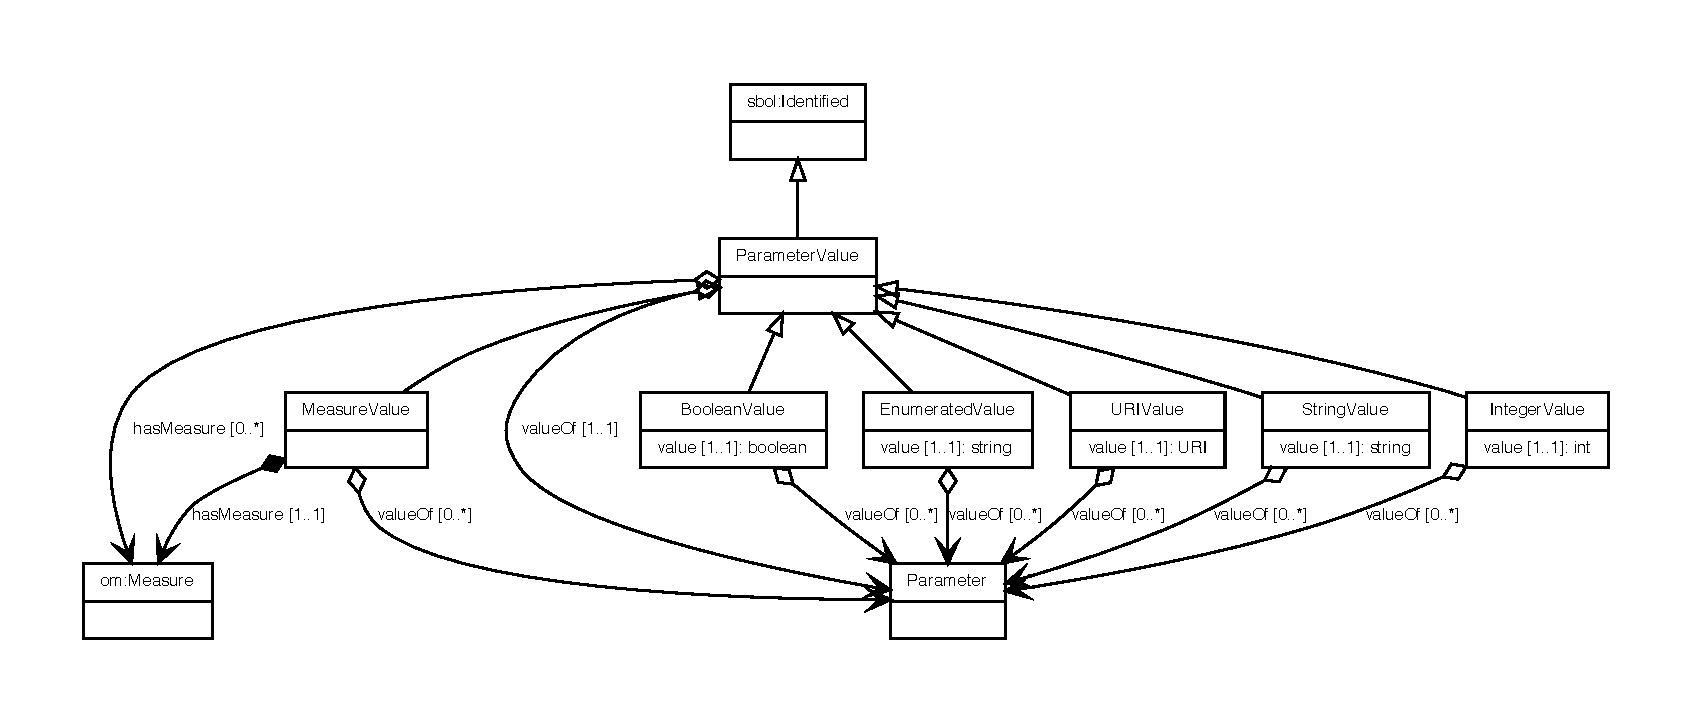
\includegraphics[scale=0.6]{figures/ParameterValue_definition_and_abstraction}
\caption[]{Diagram of the \opil{ParameterValue} abstract class and its associated properties and subclasses}
\label{uml:ParameterValue}
\end{center}
\end{figure}

\subsubsection{BooleanValue}
\label{sec:BooleanValue}

\subsubsection{EnumeratedValue}
\label{sec:EnumeratedValue}

\subsubsection{IntegerValue}
\label{sec:IntegerValue}

\subsubsection{MeasureValue}
\label{sec:MeasureValue}

\subsubsection{StringValue}
\label{sec:StringValue}

\subsubsection{URIValue}
\label{sec:URIValue}



\subsection{MeasurementType}
\label{sec:MeasurementType}

\begin{figure}[ht]
\begin{center}
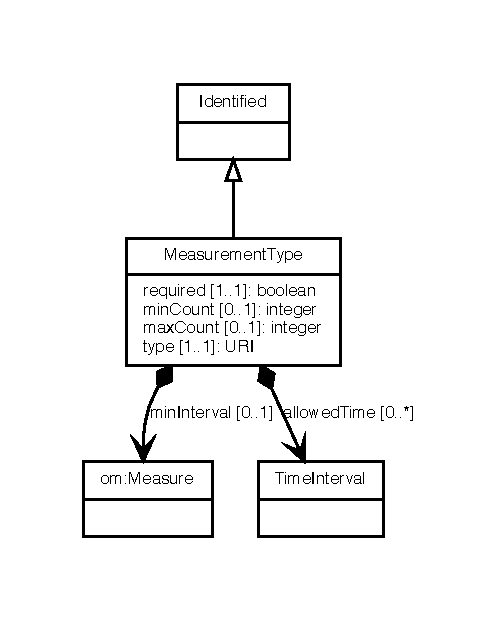
\includegraphics[scale=0.6]{figures/MeasurementType}
\caption[]{Diagram of the \opil{MeasurementType} class and its associated properties}
\label{uml:MeasurementType}
\end{center}
\end{figure}

\subsubsection{TimeInterval}
\label{sec:TimeInterval}

\begin{figure}[ht]
\begin{center}
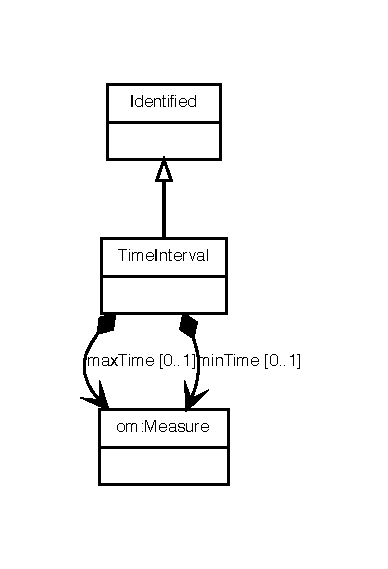
\includegraphics[scale=0.6]{figures/TimeInterval}
\caption[]{Diagram of the \opil{TimeInterval} class and its associated properties}
\label{uml:TimeInterval}
\end{center}
\end{figure}


\subsection{Measurement}
\label{sec:Measurement}

\begin{figure}[ht]
\begin{center}
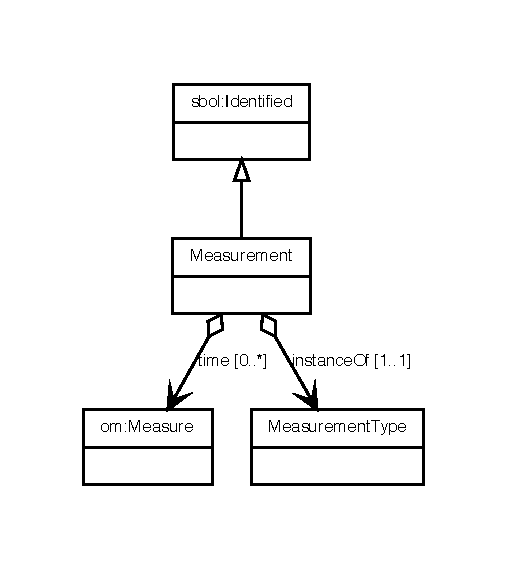
\includegraphics[scale=0.6]{figures/Measurement}
\caption[]{Diagram of the \opil{Measurement} abstract class and its associated properties}
\label{uml:Measurement}
\end{center}
\end{figure}











